\documentclass[xcolor={dvipsnames,rgb}, aspectratio=169]{beamer}

%%% PACKAGES %%%
\usepackage[T1]{fontenc}
\usepackage{tgheros}

% Metropolis customization
\usetheme[sectionpage=none]{metropolis}
\setbeamercolor{background canvas}{bg=white}
\setbeamercolor{frametitle}{bg = white, fg=black}
\setbeamertemplate{sections/subsections in toc}[square]
\setbeamertemplate{footline}{
   \textcolor{bluepoli}{\rule{\paperwidth}{1pt}}
   \vskip4pt
   \hskip5pt \tiny ODE (Pt. 2) $|$ Calcoli di Processo dell' Ingegneria Chimica
   \hskip280pt \insertframenumber
   \vskip4pt
}

% color
\usepackage{color}
\usepackage{xcolor}
\usepackage{colortbl}
\definecolor{bluepoli}{cmyk}{0.4,0.1,0,0.4}
\definecolor{mygreen}{RGB}{1, 121,111}
\definecolor{myred}{RGB}{220, 20, 60}
\definecolor{mygreen}{RGB}{28,172,0}
\definecolor{mylilas}{RGB}{170,55,241}
\definecolor{codegreen}{rgb}{0,0.6,0}
\definecolor{codegray}{rgb}{0.5,0.5,0.5}
\definecolor{codepurple}{rgb}{0.58,0,0.82}
\definecolor{backcolour}{rgb}{0.95,0.95,0.92}
\definecolor{lightblue}{rgb}{56, 167, 232}

\colorlet{colorp}{NavyBlue}
\colorlet{colorT}{WildStrawberry}
\colorlet{colork}{OliveGreen}
\colorlet{colorM}{RoyalPurple}
\colorlet{colorNb}{Plum}
\colorlet{colorIs}{black}
\newcommand{\highlight}[2]{\colorbox{#1!17}{$#2$}}
\newcommand{\highlightdark}[2]{\colorbox{#1!47}{$#2$}}

% tikz
\usepackage{tikz}
\usetikzlibrary{positioning}
\usetikzlibrary{backgrounds}
\usetikzlibrary{arrows,shapes}
\usetikzlibrary{tikzmark}
\usetikzlibrary{calc}

% tcolorbox env
% Coloured box for styling theorems, proof, definitions
\usepackage[most]{tcolorbox}

\newtcolorbox{code}[2][]{
    enhanced jigsaw,
    colframe=bluepoli,
    interior hidden, 
    breakable,
    before skip=10pt,
    after skip=10pt
}

% URL and Hyperref
\usepackage{hyperref}
\hypersetup{
    colorlinks=true,
    linkcolor=blue,
    filecolor=magenta,
    urlcolor=blue,
    pdftitle={Overleaf Example},
    pdfpagemode=FullScreen,
}
\usepackage{url}

% Math stuff
\usepackage{amsmath}
\usepackage{amssymb}
\usepackage{mathtools}
\usepackage{blkarray}
\usepackage{multirow}

% Wrapfig
\usepackage{wrapfig}

% Bibliography
\usepackage[
backend=biber,
style=alphabetic,
sorting=ynt
]{biblatex}
\addbibresource{bibliography.bib}

%%% TITLE %%%
\title{Ordinary Differential Equations\\Part 2}
\subtitle{Calcoli di Processo dell' Ingegneria Chimica}
\author[Dinelli, Mehl]{\textbf{Timoteo~Dinelli}, \textbf{Marco~Mehl}}
\institute{
   \inst{} Department of Chemistry, Materials and Chemical Enginering, G. Natta.
   Politecnico di Milano.\\
   email: timoteo.dinelli@polimi.it \\
   email: marco.mehl@polimi.it \\
}
 \date{6\textsuperscript{th} of December 2024.}

\newcommand{\norm}[1]{\left\lVert#1\right\rVert}

\begin{document}
% external files inclusion
% Double underline
\def\doubleunderline#1{\underline{\underline{#1}}}

% \newcommand{\zm}{%
%    \begin{bmatrix}
%       X_{11} & X_{12} & \cdots & X_{1p} \\
%       X_{12} & X_{22} & \cdots & X_{2p} \\
%       \vdots & \vdots & \tikzmarknode{Is}{\highlight{colorT}{X_{ij}}} & \vdots \\
%       X_{n1} & X_{n2} & \cdots & X_{np} \\
%    \end{bmatrix}%
% }

\makeatletter
\newcommand{\DrawLine}{%
  \begin{tikzpicture}
  \path[use as bounding box] (0,0) -- (\linewidth,0);
  \draw[color=bluepoli,dashed,dash phase=2pt]
        (0-\kvtcb@leftlower-\kvtcb@boxsep,0)--
        (\linewidth+\kvtcb@rightlower+\kvtcb@boxsep,0);
  \end{tikzpicture}%
  }
\makeatother

{%
   \setbeamertemplate{footline}{}
   \begin{frame}{}
      \maketitle
      \begin{tikzpicture}[overlay, remember picture]
         \node[above left=6.5cm and .01cm of current page.south east] {
         \includegraphics[trim=1cm 1cm 1.5cm 1cm, clip=true, width=6cm]{
            ./../../Introduction to Matlab/slides/figures/_static/ING_IND_INF-eps-converted-to.pdf
         }
      };
      \end{tikzpicture}
   \end{frame}
}

%%%%%%%%%%%%%%% EXERCISES
{%
   \setbeamertemplate{footline}{}
   \begin{frame}[standout]
	   Exercises
   \end{frame}
}

\begin{frame}{Exercises}
   \begin{itemize}
      \item[$\blacktriangleright$] \textbf{Exercise 1 \textcolor{red}{Available on Matlab
         GRADER}}: \small{A batch reactor is employed to facilitate a biological process,
         wherein the growth of a biomass (B) and the loss of substrate (S) occur
         concurrently. The objective is to ascertain the dynamics of both B and S over a
         15-hour period, while attempting to vary the parameters for the purpose of error
         control in the ordinary differential system. This will be achieved by adopting a
         relative tolerance of $10^{−8}$ and an absolute one of $10^{−12}$ (with respect
         to the default Matlab values). The ODE system that describes the evolution of
         the process is presented below:}
         \begin{equation*}
            \begin{cases}
               \frac{dB}{dt} = \frac{k_{1} \times B \times S}{k_{2} + S} \\
               \frac{dS}{dt} = -k_{3} \times \frac{k_{1} \times B \times S}{k_{2}+S} \\
               B(0) = 0.03 \frac{kmol}{m^{3}}\\
               S(0) = 4.5 \frac{kmol}{m^{3}}
            \end{cases}
         \end{equation*}
         Where: $k_{1} = 0.5 h^{-1}$, $k_{2} = 10^{-7} \frac{kmol}{m^{3}}$, $k_{3} =
         0.6$.
   \end{itemize}
\end{frame}

\begin{frame}{}
   \begin{itemize}
      \item[$\blacktriangleright$] \textbf{Exercise 2 \textcolor{red}{Available on Matlab
         GRADER}}: \small{A perfectly mixed heated tank is subjected to a step
         disturbance in the inlet temperature, occurring at $t=150 \: s$ with an increase
         of $30 \: ^{\circ}C$. The objective is to evaluate the dynamics of the outlet
         temperature subsequent to the step disturbance, assuming a steady-state regime
         for the liquid level in the tank. The data are as follows: The heat transfer
         coefficient is $Q = 1 \:MW$, the inlet flow rate is $F_{in} = 8 \: kmol/s$, the
         mass is $m = 100 \: kmol$, the specific heat capacity is $Cp = 2.5 \:
         kJ/kmol/K$, and the inlet temperature is $T_{in} = 300 \: K$. The associated
         system of equations is as follows:}

         \begin{equation*}
            \begin{cases}
               \frac{dT}{dt} = \frac{Q}{mCp} - \frac{F_{in}}{m}\left(T-T_{in}\right) \\
               F_{in} = F
            \end{cases}
         \end{equation*}
   \end{itemize}
\end{frame}

\begin{frame}{}
   \begin{itemize}
      \item[$\blacktriangleright$] \textbf{Exercise 3}: \small{The objective is to
         evaluate the height dynamics of a single cylindrical tank subjected to a step
         disturbance on the inlet flow rate, whereby the flow rate is reduced to half of
         its initial value. Additionally, the height dynamics of the tank are to be
         evaluated after a linear decrease in the inlet flow rate, occurring over a
         period of 30 seconds, whereby the flow rate is reduced to half of its initial
         value. The data are presented below: The area of the tank is 30 $m^2$, the
         initial flow rate is 7.5 $m^3 / s$, the outflow is proportional to the height
         divided by the radius, and the radius is 0.4 $m$. The associated system of
         equations is as follows:}
         \begin{equation*}
            \begin{cases}
               \frac{dh}{dt} = \frac{F_{i}}{A} - \frac{h}{Ar} \\
               F_{i} = F_{i}^{0}/2 \\
               h(0) = h_{ss} = r \times F_{i}^{0} = 3
            \end{cases}
         \end{equation*}
         \small{The second request of the exercise is analogous to the first. The only
         distinction is in the perturbation of the inlet flow rate, which now follows a
         linear decrease occurring in 30 seconds.}
   \end{itemize}
\end{frame}

\begin{frame}{}
   \begin{itemize}
      \item[$\blacktriangleright$] \textbf{Exercise 4 \textcolor{red}{Available on Matlab
         GRADER}}: \footnotesize{Two tanks are positioned in succession, and the two
         tanks can be arranged in two distinct configurations: the "{\it
         non-interacting}" and the "{\it interacting}". It is evident that the flow rate
         exiting the initial tank will influence the subsequent tank's behavior in the
         event of a disturbance. However, in the case of the interacting tank, the flow
         rate exiting the second tank will also affect the behavior of the first tank.
         The data are presented below: The areas of the tanks are 30 m$^2$ and 50 m$^2$,
         respectively. The rates of outflow from the tanks are 1.2 and 0.7 $m^2 /s$,
         respectively. The initial volume of the fluid in each tank is 9.4 m$^3$.}
         \begin{columns}
         \column{0.5\textwidth}
            \centering
            \textbf{Non Interacting tanks}:
               \begin{equation*}
                  \begin{cases}
                     \frac{dh_{1}}{dt} = \frac{F_{i} - \frac{h_{1}}{r_{1}}}{A_{1}} \\
                     \frac{dh_{2}}{dt} = \frac{\frac{h_{1}}{r_{1}} - \frac{h_{2}}{r_{2}}}{A_{2}} \\
                     h_{1}(0) = 11.28 \\
                     h_{2}(0) = 6.58
                  \end{cases}
               \end{equation*}
         \column{0.5\textwidth}
            \centering
            \textbf{Interacting tanks}:
            \begin{equation*}
               \begin{cases}
                  \frac{dh_{1}}{dt} = \frac{F_{i} - \frac{h_{1} - h_{2}}{r_{1}}}{A_{1}} \\
                  \frac{dh_{2}}{dt} = \frac{\frac{h_{1}-h{2}}{r_{1}} - \frac{h_{2}}{r_{2}}}{A_{2}} \\
                  h_{1}(0) = 17.86 \\
                  h_{2}(0) = 6.58
               \end{cases}
            \end{equation*}
         \end{columns}
   \end{itemize}
\end{frame}

\begin{frame}{}
   \begin{itemize}
      \item[$\blacktriangleright$] \textbf{Exercise 5}: \small{The following two
         elementary liquid-phase reactions are conducted in an adiabatic manner within a
         10 $L$ plug flow reactor:}
         \begin{equation*}
            \begin{cases*}
               A+2B\longrightarrow2C \quad \Delta H_{1} = 20000\frac{cal}{mol}  \quad
               k_{1} = 0.001\frac{L^{2}}{mol^{2}\:s}@ 300K \quad E_{1} = 5000\frac{cal}{mol} \\
               A+C\longrightarrow2D \quad \Delta H_{2}  = -10000\frac{cal}{mol} \quad
               k_{2} = 0.001\frac{L}{mol\:s}@ 300K \quad E_{2} = 7500\frac{cal}{mol}
            \end{cases*}
         \end{equation*}
         \small{Once streams A and B have been combined, species A is introduced into the
         reactor at a concentration of $CA_{0} = 2 mol/L$, while species B is introduced
         at a concentration of 4 $mol/L$. The total volumetric flow rate at the point of
         entry is 10 $L/s$. If the entering temperature were adjustable between 600 $K$
         and 700 $K$, which entering temperature would be recommended to maximize the
         concentration of species C exiting the reactor, with an accuracy of $\pm$10 $K$?
         It is assumed that all species have the same density and that there is a
         negligible pressure drop along the reactor.}
   \end{itemize}
\end{frame}

\begin{frame}{}
   \begin{itemize}
      \item[ ]
         \begin{equation*}
            \begin{cases}
               \frac{dF_{A}}{dV} = -r_{1} - r_{2} \\
               \frac{dF_{B}}{dV} = -2r_{1} \\
               \frac{dF_{C}}{dV} = 2r_{1} - r_{2} \\
               \frac{dF_{D}}{dV} = 2r_{2} \\
               \frac{dT}{dV} = \frac{-r_{1}\Delta H_{1} - r_{2}\Delta H_{2}}{\sum F_{j}Cp_{j}}
            \end{cases}
         \end{equation*}
         Where:\\
         $r_{1} = k_{1}C_{A}C_{B}^{2}$; $r_{2} = k_{2}C_{A}C_{C}$\\
         $K1=k_{1}^{ref}exp\left[-\frac{E_{1}}{R}\left(\frac{1}{T}-\frac{1}{T_{ref}}\right)\right]$;
         $K2=k_{2}^{ref}exp\left[-\frac{E_{2}}{R}\left(\frac{1}{T}-\frac{1}{T_{ref}}\right)\right]$\\
         $C_{A} = F_{A}/Q_{0}$, $C_{B} = F_{B}/Q_{0}$, $C_{C} = F_{C}/Q_{0}$.
   \end{itemize}
\end{frame}

\begin{frame}{}
   \begin{itemize}
      \item[$\blacktriangleright$] \textbf{Exercise 6}: \footnotesize{A mass is attached
         to a spring dumper system. The temporal evolution of its relative position can
         be described by means of a second-order differential equation.
         \begin{equation*}
            \frac{d^2 z}{dt^2} = g - \frac{kz}{m} - \frac{cv}{m}
         \end{equation*}
         The second-order equation can be reformulated as a system of two ordinary
         differential equations as follows:
         \begin{equation*}
            \begin{cases}
               \frac{dz}{dt} = v \\
               \frac{dv}{dt} =  g - \frac{kz}{m} - \frac{cv}{m}
            \end{cases}
         \end{equation*}
         Where: $m = 1 \: kg$, $g = -9.81 \: m^2 /s$, $k=10 \: N/m$, $c=1\: N\:s/m$, $z_0
         = 0\: m$.}
   \end{itemize}
   \begin{figure}
      \centering
      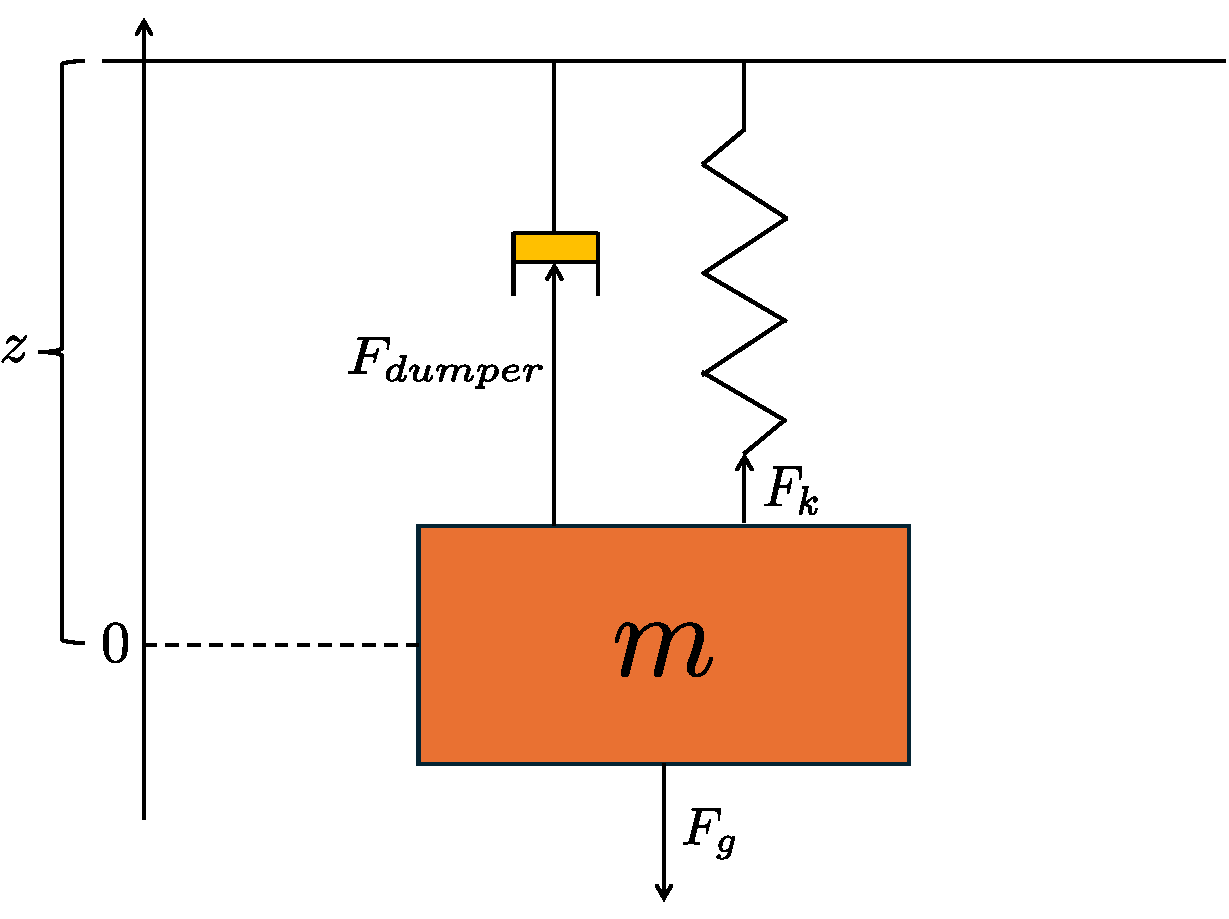
\includegraphics[width=0.3\textwidth]{figures/MassSpringDumper.pdf}
   \end{figure}
\end{frame}

%%%%%%%%%%%%%%% CLOSING
{%
\setbeamertemplate{footline}{}
\begin{frame}[standout]
	Thank you for the attention!
\end{frame}
}

\end{document}
